\documentclass[12pt,a4paper, oneside]{article}
\usepackage{hyperref}
\usepackage{geometry}
\usepackage[light,math]{iwona}
\usepackage{amsmath}
\usepackage{hyperref}
\usepackage{pdfpages}
\newcounter{includepdfpage}
\usepackage[toc,page]{appendix}
\usepackage{setspace}
\usepackage{amsfonts}
\usepackage{amssymb}
\usepackage{graphicx}
\usepackage{pgfplots}
\usepackage{gnuplot-lua-tikz}
\usepackage{mdframed}
\usepackage{epstopdf}
\epstopdfsetup{outdir=./}
\usepackage{float}
\usepackage{parskip}
\usepackage{fancyhdr}
\renewcommand{\footrulewidth}{0.4pt}
\usepackage{color}
\usepackage{multirow}
\definecolor{MyColor}{rgb}{0.8, 0.8, 0.8}
\definecolor{darkgreen}{rgb}{0, 0.4, 0}
\definecolor{ugentblue}{rgb}{0.05,0.18,0.37}
\usepackage{colortbl}
\newlength{\drop}
\newcommand{\todo}[1]{{\color{red}\textbf{(TODO: #1)}}}
\usepackage[super]{nth}
\usepackage{rotating}
\usepackage{tabularx}
\usepackage{amsmath}
\usepackage{graphicx}
\usepackage{tikz}
\usepackage{fancyhdr}
\usepackage{dsfont}
\usepackage{parskip}
\usepackage{epstopdf}
\usepackage{listings}
\usepackage{color}
\definecolor{lichtgrijs}{gray}{0.95}
\usepackage{natbib}
\bibliographystyle{plain}
\usepackage[nottoc]{tocbibind}
\usepackage[justification=centering,bf,hang]{caption}
\usepackage{pgfplots}
\usepackage{import}
\pgfplotsset{compat=newest}
%\usepackage{subfig}
\usepackage{textcomp}
\usepackage{array}
\usetikzlibrary{arrows,automata}
\usepackage{float}
\usepackage{longtable}
\usepackage{titling,enumitem}
\usepackage{a4wide}
\usepackage{amssymb}
\usepackage{rotating}
\usepackage{listings}
\usepackage{titling}
\usepackage{blindtext}
\usepackage{chngpage}
\usepackage{calc}
\usepackage{array}
\usepackage[toc,acronym,ucmark]{glossaries}
\usepackage{lstautodedent}
\newcolumntype{L}[1]{>{\raggedright\let\newline\\\arraybackslash\hspace{0pt}}m{#1}}
\newcolumntype{C}[1]{>{\centering\let\newline\\\arraybackslash\hspace{0pt}}m{#1}}
\newcolumntype{R}[1]{>{\raggedleft\let\newline\\\arraybackslash\hspace{0pt}}m{#1}}

\newcolumntype{Y}{>{\raggedleft}p{0.50\textwidth}}
\newcolumntype{Z}{p{0.8\textwidth}}
\lstset{ %
  backgroundcolor=\color{white},   % choose the background color; you must add \usepackage{color} or \usepackage{xcolor}
  basicstyle=\scriptsize\ttfamily,        % the size of the fonts that are used for the code
  breakatwhitespace=false,         % sets if automatic breaks should only happen at whitespace
  breaklines=true,                 % sets automatic line breaking
  captionpos=b,                    % sets the caption-position to bottom
  deletekeywords={...},            % if you want to delete keywords from the given language
  escapeinside={\%*}{*)},          % if you want to add LaTeX within your code
  extendedchars=true,              % lets you use non-ASCII characters; for 8-bits encodings only, does not work with UTF-8
  frame=single,                    % adds a frame around the code
  keepspaces=true,                 % keeps spaces in text, useful for keeping indentation of code (possibly needs columns=flexible)
  keywordstyle=\color{blue},       % keyword style
  language=PYTHON,
  otherkeywords={*,...},            % if you want to add more keywords to the set
  numbers=left,                    % where to put the line-numbers; possible values are (none, left, right)
  numbersep=5pt,                   % how far the line-numbers are from the code
  rulecolor=\color{black},         % if not set, the frame-color may be changed on line-breaks within not-black text (e.g. comments (green here))
  showspaces=false,                % show spaces everywhere adding particular underscores;cite it overrides 'showstringspaces'
  showstringspaces=false,          % underline spaces within strings only
  showtabs=false,                  % show tabs within strings adding particular underscores
  stepnumber=2,                    % the step between two line-numbers. If it's 1, each line will be numbered
  tabsize=2,                       % sets default tabsize to 2 spaces
  title=\lstname                   % show the filename of files included with \lstinputlisting; also try caption instead of title
}

\usepackage[nottoc]{tocbibind}				% add bibliography to table of contents
\usepackage{graphicx}
\usepackage{caption}
\usepackage{subcaption}

\makeatother
\makeglossaries
%!TEX root=report.tex
\newacronym{kdc}{KDC}{Key Distribution Center}
\newacronym{vpn}{VPN}{Virtual Private Network}
\newacronym{ddos}{DDoS}{Distributed Denial of Service}
\newacronym{nist}{NIST}{National Institute of Standards and Technology}
\usepackage{hyperref}
\hypersetup{
    pdfauthor = {Eveline Hoogstoel, Wouter Pinnoo, Stefaan Vermassen and Titouan Vervack},
    pdftitle = {Information Security Assignment},
    pdfsubject = {},
    pdfkeywords = {}
}

\author{Eveline Hoogstoel \and Wouter Pinnoo \and Stefaan Vermassen \and Titouan Vervack}
\date{May 2016}
\title{Information Security Assignment}

\begin{document}

\newgeometry{top=1.5cm, right=1.70cm, left=1.7cm}
\begin{titlepage}

\pagenumbering{Alph}
\begin{figure}[!ht]
  \begin{adjustwidth}{-\oddsidemargin-1in}{-\rightmargin}
    \centering
    
\includegraphics[width=\paperwidth]{assets/banner}
  \end{adjustwidth}
\end{figure}
\vspace{-0.2em}
\begin{center}
\vspace{7cm}
\Huge \textbf{Information Security Assignment\\\LARGE{Security for a (Car) Key App}\\\Large{Report}}\\
\vspace{6.0cm}
\large
\begin{tabular}{Y! {} Z}
& {\bf Academic year 2015-2016} \\
& \\
& {\bf Group 1} \\
&\\
& {\bf Eveline Hoogstoel} \\
& {\bf Wouter Pinnoo} \\
& {\bf Stefaan Vermassen} \\
& {\bf Titouan Vervack} \\
\end{tabular}
\end{center}
\end{titlepage}
\pagenumbering{arabic}

\restoregeometry
\newgeometry{top=1in, bottom=1in, left=.8in, right=.8in}

\pagestyle{fancy}
\fancyhf{}
\lhead{Information Security Assignment}
\rhead{Group 1}
\cfoot{\thepage}

\clearpage
\tableofcontents
\clearpage
\section{Introduction}
\subsection{Problem statement}
Companies with business in car rental services, or companies looking for a digitalisation of the keys or their company cars, can opt to use a system where drivers can book, (un)lock and start a pre-booked car using a smartphone application. In this assignment, the security aspect of this use case is designed and a prototype is presented that illustrates a working implementation of the designed security mechanisms. Sequence diagrams and an UML diagram of the prototype can be found in Appendix \ref{appendix}.

\subsection{Requirements}
The design of our system will be made with a number of requirements in mind. First of all, simplicity is important to minimise unneeded delays and thus not harming the availability requirement of our system. Although distributed attacks such as \gls{ddos} attacks are very hard to avoid in its entirety, some measures will be taken in the proposed system to ensure a reasonable availability. Availability is very important for the users of the system since large delays when, for example, opening a car will be experienced as main weaknesses of the system. Also, the system must be able to operate when the network coverage can occasionally not be assured. However, a few assumptions about network coverage will be made in Section \ref{sec:system-description}.\par
A second requirement is authentication. The system should protect thieves from impermissible usage of company cars, and will thus have to make sure only authorised users have access to cars they have booked.\par
Next, all communication that is vulnerable to eaves-dropping (e.g. communication via a public insecure communication network) or any other kind of misuse, will have to be protected to ensure confidentiality. It must be impossible for an intruder to capture classified information (such as personal information).\par
Finally, data-integrity and non-repudiation are important requirements. The former states that any modifications made on message sent over the (public) communication network will cause the other party to detect that the message is altered. The latter ensures that neither sides of the communication network can question the data-origin validity of a message. One of the reasons that this is an important requirement is that users will actually be billed for the usage of the company cars --- after a billing statement is sent, one must not be able to reasonably argue the contents of the bill.


\section{System description}\label{sec:system-description}
First, a short overview of the general architecture of the system will be given. Next, the functionalities and general security mechanisms of each module will be explained.
\subsection{Architecture overview}
The system we propose consists of three parts: the server, the user and the car. The server will run different modules, i.e., the \textit{booking} module, the \textit{billing} module and the \textit{car communication} module. Each module and its corresponding functionality will be explained in Section \ref{sec:server-modules}. \par
An overview of the whole system is depicted in Figure \ref{fig:architecture}. The car will need to send/receive messages to/from the server. For these communications we prefer to use 4G technology, because we have no guarantee that the car has Wi-Fi available and the coverage of 4G is bigger. The user will need to communicate, by using our smartphone application, with the car to identify himself. This communication will happen via NFC. We assume that modern smartphones have an NFC-chip.

\begin{figure}[H]
\centering
\includegraphics[width=0.8\textwidth]{assets/architecture}
\caption{General overview of the architecture.}
\label{fig:architecture}
\end{figure}

\subsection{Server modules}\label{sec:server-modules}
The server consists of following modules:
\begin{itemize}
\item \textit{Booking module}: responsible for booking a car, based on communication between the smartphone application and the server.
\item \textit{Car communication module}: a part of the server that communicates with the cars.
\item \textit{Billing module}: the part of the server that calculates billing details and sends the bills to the users.
\end{itemize}
These modules were developed separated to increase modularity, so that eventually a module can be moved to other servers. Also, the server could be configured to assign computation power to the module that needs it the most (and for example idling the billing module since its activities don't have to be performed in real-time). In our prototype, all modules will run on the same simulated server, so this server has one private-public key pair. We assume that the public key of the server is available to the cars and the smartphone applications. This can be done by simply hard-coding it in the software. Should the public key be compromised, no security risks will come up because no data can be decrypted without the private key. Also, there's no loss of data-origin guarantee because every message that will be sent to the server will be signed with either the private key of the user or the private key of the car.

\subsubsection{Booking module}\label{sec:booking-module}
The booking module will be used to receive booking requests from the smartphone application. It will notify the car communication module when a new booking is requested and approved.  We assume that these different modules are located on the same server, so that no network hacking can harm the connection between the modules.
\par
In this module, we focus on authentication and confidentiality. We have to be sure that nobody can issue a booking request for another user. The request should also be received untampered at the server and no man in the middle should be able to read the actual contents of the booking request.

\subsubsection{Car communication module}\label{sec:cc-module}
The car communication module will be used to send booking information to the car and to receive billing information from the car. This module will ensure that the communication between the car and the server is secure, since this communication will happen via an untrusted and open network. This module will receive information from the booking module and send the billing information to the billing module. We assume that these different modules are located on the same server, so that no network hacking can harm the connection between the modules.
\par The first security service the car communication module has to implement is confidentiality. If the messages are not encrypted an attacker could eavesdrop the network and read the messages. To encrypt our messages we will make use of AES encryption. The car or the car communication module will generate an AES key before starting the communication. This key will be exchanged before the communication starts. The second security service we have inspected is authentication, since the information send between car and \textit{car communication module} is sensitive and we want to prevent a replay attack. Each message will be signed with the private key of the sender.

\subsubsection{Billing module}\label{sec:billing-module}
The billing module is a part of the server that is located on the same server as the \textit{Car communication module}.\par
Since the communication between the car and the \textit{car communication module} will be secured, and this module is located on the same server as the \textit{billing module}, the billing does not have to take additional security precautions. The billing module is only responsible for calculating the amount to bill to the user.

\subsection{Car}
The module in the car will have the following tasks:
\begin{itemize}
\item[--] Decide if the car can be opened.
\item[--] Decide if the car may be started.
\item[--] Store billing information in a buffer.
\item[--] Store booking information temporarily.
\item[--] Communicate with the car communication module.
\end{itemize}

All cars that are involved in the system will need to be in possession of a smart card. This smart card will be used to store some information, to communicate with the server and to send signals to the car.
We decided to use a smart card in the car for the following reasons \citep{smartcard}:
\begin{enumerate}
\item Authentication: The smart card is embedded by a unique private key which is generated by the manufacturer of the smart card.
\item Strong device security: The smart card is extremely difficult to duplicate. Smart cards are designed in a way that they detect and react to tampering attempts. 
\end{enumerate}
So, with the use of the smart card a malicious user is not able to retrieve the private key. Therefore, we can state that the private key of the car is a unique and secure identifier for the car, so the car can use this for authentication purposes.

Since a car needs to be able to communicate with the server, the smart card will be integrated with a SIM-card. This allows the communication to occur via a mobile network. A cellular network has large coverage but in some places there is no network available, for instance in a parking lot. Therefore the car needs to have some memory available, where he can store information temporarily. For instance, the booking information will be send to the car a few days before the booking and when the trip is finished the car will calculate the billing information and store it in memory until he is able to send it to the server. To store some information the smart card will need 28 bytes per booking entry and 32 bytes per billing entry. If we assume that the server is sending the booking information only 5 days upfront and a car is booked for 5 days every hour, then this information is 3360 bytes. The billing information will be calculated after the trip and will be send to the server when a network is available. We assume that during the next trip, the car will be able to send the information to server, so at most one billing entry will be stored on the smart card. We can conclude that 4 kB of memory is sufficient to store the booking and billing information.

\subsection{Smartphone Application}\label{sec:user}
The smartphone application will be responsible for the following tasks:
\begin{itemize}
\item[--] Register a user
\item[--] Book a car
\item[--] Issue a command to the car (start, stop, (un)lock car)
\end{itemize}

This requires that the smartphone application has an internet connection when it is registering and when it is booking a car. To be able to communicate with the Car it will need to have an NFC connection.

To be able to communicate with the server (for registration and booking), the public key of the server is hard-coded into the application. When we need to commence communication, the application will generate an AES key and encrypt it with the server's public key and send this to the server. The server and the application then both know the AES key and can securely communicate with one another.

To be able to communicate with the car, we do the same thing. During booking, we received the public key of the car. Using this key we do another AES key exchange with the car, as done before with the server. Now that the car and the application both know the same AES key they can securely communicate with one another.

We assume that the smartphone application runs inside of a sandbox and is not able to be hacked from the phone itself (e.g. a virus reads the applications' memory, retrieving an AES key, which can then be send to the creator of the virus which might then be able to open the car at a later date as it has the required key for communication). Further more we assume that the private key and UID of the application remain secret as compromising these would allow a malicious user to set up a secure connection. Several Android implementations exist that can secure internal storage \cite{6341374, cooijmans2014secure}.

\subsection{Use cases}\label{sec:usecases}
\subsubsection{Smartphone-server communication}
For the communication between the app and server, we will use a mobile network technology, such as 4G or WiFi. Customers can use this application wherever they want. We make the assumption that packets always reach the server, although it is possible that packets are sniffed and replayed. 
\par
When we focus on confidentiality, we should consider man-in-the-middle attacks. An example of this sort of attacks is eavesdropping where packets are intercepted by the attacker. To prevent this attack, all packets need to be encrypted. If the message can be intercepted by the attacker, he can not retrieve the actual contents. Booking data will be encrypted using AES, which will use a key that is uniquely generated by the application for each transmission. As the application will generate the AES key, a key exchange process is compulsory. For this purpose, RSA will be used.
\subsubsection{Registration}
When a customer downloads the application, a registration is necessary. During the registration, the customer will be assigned a userID and his/her driver's license will be validated. The server's public key will be hardcoded in the smartphone application. This imposes no security risk: only the server knows his private key and everyone may send encrypted data to the server. If the server's private key would become compromised, it is sufficient to roll-out a mandatory application update with the new public key built-in.
\par
To start the registration, an AES key will be generated by the application. The AES key will then be encrypted using the server's public key. This message will be send to the server. For this purpose, no measures against replay attacks are necessary. Everyone may issue a registration request to the server and no user-specific data is included in this message.
If the server receives this message, it will decrypt it using its own private key and generate a userID. This userID will be signed using the server's private RSA key. PKCS1-1.5 is used in this encryption to enforce structure. This way, the application can verify the identity of the server by decrypting the message using the AES and checking the PKCS structure. 
\par
To be able to perform a secure AES key exchange for an existing user, the server needs to know the application's public key to verify the identity in the key exchange process. For this purpose, the application will generate a new private/public key pair one time during the registration. The public key will be sent using the AES key, generated in the first step of this process. Also the userID will be added to the message, as the server has to look up the corresponding AES key to decrypt the message containing the application's public key.
\par
From now on, we can issue an AES key exchange for each transmission, to ensure freshness of the AES key. This process is discussed in Section \ref{sec:keyexchange}. After the key is negotiated, the registration info, including the driver license, will be send to the server using AES encryption. Here again PKCS1-1.5 will be used. However, the server needs to determine which AES key to use, as it has one for every customer. For this purpose, the userID will also be send. This will be done using RSA encryption, to prevent disclosure or adjustments by an attacker, where he would try to assign the registration info to another user. The attempt can for instance be to link a valid driver's license to a user that doesn't have one. When the server receives the registration info, the existing AES key will be erased from the temporary dictionary.  

\subsubsection{Key Exchange}
\label{sec:keyexchange}
The key exchange process is shown in Figure \ref{fig:sequencediagram-keyexchange}. To start the process, an AES key is generated by the smartphone application. The AES key is then encrypted using the app's private RSA key. PKCS1-1.5 is used in this encryption to enforce structure. This way the server can verify the identity of the application by decrypting the the AES key and checking the PKCS structure. For this purpose, the server also needs the userID, which will also be added to the message. Next to the userID and the AES key, also a timestamp will be included in the message. The reason for this, is to prevent replay attacks, where the attacker re-sends old valid messages to the server. Using timestamps, one can validate the freshness of the message by checking the timestamp against its own clock. When the timestamp, adjusted with some possible skew, differs to much from the server time, the attack is detected.
The whole message is encrypted using the server's public key, so the server is the only entity that can read the actual content of the message by decrypting it with its own private key. 
\par
When the server receives the message, it will decrypt it using its own private key and check the timestamp. The server will then look up the app's public key, that it has received during the registration process. For this purpose, the userID is used, as the public keys are stored in a dictionary where userIDs are mapped on public keys. It will then decrypt the AES key and verify the PKCS structure to verify the app's identity. If this is successful, the AES key will be linked to the corresponding user ID in a temporary dictionary.
\par
The AES key will be used by the application to send data to the server. When the server receives this data, the AES key will be erased from the dictionary and a new key exchange is necessary. The AES key is valid for only one data transfer. The advantage is that if the AES key would become compromised, this forms no security risk. The disadvantage is that a key exchange is necessary for each data transfer. As we assume that bookings are done at most  a few times a day, this overhead is negligible. However,  this AES key could even be reused for several days without imposing a serious security risk. 
\par
We have taken appropriate measures against replay attacks, using timestamps, and eavesdropping, as the message is encrypted using the server's public key. Hackers may try to assign fake AES keys to victims by sending fake request. However, since we have signed the AES key using the app's private key, these attacks will be detected. Attackers don't possess  the private key of the application and the message is structured using the PKCS scheme. 
\par
If a request fails, the server will send no error messages back to the transmitter to prevent information leakage.

\subsubsection{Booking}\label{sec:booking}

A booking request will always start with an AES key exchange, discussed in Section \ref{sec:keyexchange}. After the key is negotiated, the booking info will be send to the server using AES encryption. Here again PKCS1-1.5 will be used. However, the server needs to determine which AES key to use, as it has one for every customer. For this purpose, also the userID will be sent. This will be done using RSA encryption, to prevent disclosure or adjustments by an attacker, where he would try to assign the booking request to another user. 
\par
By using AES encryption, with an AES key that is only known by the application and the server, we can ensure non-repudiation. Only the client can send data using the correct userID and AES key combination. If the attacker sends malicious requests to the server, the AES encrypted data can not be decrypted as it doesn't posses the right AES key. We have also taken measures against replay attacks by adding timestamps to the messages. When the timestamp, adjusted with some possible skew, differs too much from the server time, the attack is detected.

After the booking module confirmed the booking it will sends the booking info back to the smartphone application, for viewing purposes, and because the smartphone needs the booking id and public key of the car to be able to successfully communicate with the car as is explained in Section \ref{sec:unlocking-starting-car}. This information is once again exchanged by encryption with an AES key that has been obtained from a new key exchange between the server and the smartphone application.

The carcommunication module gets a notification of a new booking from the booking module and will buffer this information. When a network is available to the car, the carcommunication module sends an update of the new bookings. First a key exchange needs to be performed, to negotiate an AES key. This process is analogue to the process shown in Figure \ref{fig:sequencediagram-keyexchange}, but acts between the car and the car communication module. After the key exchange the car communication module sends the booking info encrypted with the AES key to the car. The car communication module will also add a timestamp in the message to prevent a replay attack.

\subsubsection{(Un)locking and starting the car}\label{sec:unlocking-starting-car}
\par This use case illustrates multiple actions as the security measures needed for the actions are the same. When a user wants to (un)lock or start a car, we have to be certain that he is the legitimate user who booked the car, so authentication is needed. Next to authentication, confidentiality is needed to prevent eavesdropping (even though this is not the easiest task in the case of NFC), especially to be able to support technologies other than NFC in the future. Even though eavesdropping has been prevented by confidentiality, we also have to protect against replay attacks by using a timestamp or sequence number. A sequence diagram depicting the interactions in this usecase can be found in Figure \ref{fig:sequencediagram-carcommands}.

\par The car has already received the booking information through the \textit{car communication module} (see Section \ref{sec:cc-module}), this information includes the public key of the smartphone application and the time interval during which the user is able to use the car. The smartphone application acquired the public key of the car during the booking (see Section \ref{sec:booking}).

\par When the user issues a start, stop or (un)lock command (in Step 1), an AES key exchange between the smartphone and the car is started over NFC (see Step 2). To be certain that no one other than the legitimate user sets up a secure connection, the exchange contains a timestamp that is encrypted with the smartphone app's private key. This ensures authenticity, confidentiality and protects against replay attacks.

\par We then create a message that contains the command  appended by the booking id (to verify booking information) and a timestamp to prevent replay attacks, this is what you see in Step 3. We do not sign this message because we know you are the legitimate user due to the authentication that happened in the AES key exchange. If you did not adhere to authentication during this key exchange, you could not have set up this secure connection. In Step 4 this message is then encrypted with the AES key to prevent eavesdropping. The message is then send to the car in Step 5.

\par When the car receives the message it will decrypt the message using the AES key it received in the key exchange with the smartphone application, as shown in Step 6. The car then checks if the timestamp is correct (within 100ms of the current time). Finally, it will check if the booking id corresponds with the currently active booking. In case everything is correct, the command will be executed as depicted in Step 7.\\

\par In case the car is locked, the billing will be processed by the \textit{billing module}, as is explained in the next section, Section \ref{sec:usecase-billing}.

\subsubsection{Billing}\label{sec:usecase-billing}
As discussed in Section \ref{sec:unlocking-starting-car}, every time the user locks a car, a command is sent to the car. If the car detects that the command was to lock the car, the \textit{billing} use case is initiated, which is briefly discussed in this section and depicted in Figure \ref{fig:sequencediagram-billing}.\par


Once the car receives the command to lock the car, it stores data about the finished trip (travelled distance, duration, etc.) in step 1. In step 2, a key exchange between the car and the \textit{car communication module} on the server is initiated, so that they both have an AES key that can be used for the encryption of the transfer of the billing data (trip data: travelled distance, duration, etc.). This AES key exchange is similar to that described in Section \ref{sec:booking}: the only difference is that the Car UID is used instead of a User UID. Once both parties (the car and the server) have knowledge of the AES key, the trip data, along with a timestamp and the Car UID is transferred in step 5. The server uses its stored AES key to decrypt the message and checks whether the message is still valid with the timestamp. If this can be verified, the billing information is passed to the \textit{billing module}, which processes the bill and sends it to the user via mail.

\subsection{Technical decisions}\label{sec:technical-decisions}

\subsubsection{Keylengths}
For RSA, a key length of 2048 bits is used, which allows for 112 bits of security strength. A recent study of the US \gls{nist} \cite{Publication2007} (January 2016) indicates that this security strength will still be safe through 2030. Encryption of new data from 2031 and beyond however, will be disallowed to use a security strength of 112. Instead, a security strength of 128 bits (RSA 3072) should be used from 2031 and beyond. We conclude that a compatibility until 2030 is sufficiently long, especially for a prototype of a system that is currently not common on the market of car security. Hardware implementations in the car will probably have changed earlier than 2030.\par
In case the key length should be changed, the proposed proof-of-concept system will not work anymore. Not only the server software and smartphone application will have to be updated, the smartcards inside the cars will have to be replaced. With ease-of-use in mind, the proof-of-concept system can be adapted to detect version changes such that cars with old smartcards will automatically stop working when the key length is updated, or the smartphone application will force the user to update the application for further usage.\par
The used library for AES key generation (the Java Crypto library) uses a default AES key length of 128 bits. According to \cite{Publication2007}, an AES key length of 128 bits will even be acceptable after 2030.\par
Of course, when stating that the proposed key length of 2048 bits is sufficiently strong until 2030, we assume no quantum computer algorithms are used. If that should be the case, a length of 2048 is probably not safe until 2030. Especially the RSA keys will be vulnerable and will have to be extended. However, although some algorithms already exist for quantum computing attacks, probably computers capable of running such algorithms on 2048-bit keys will not exist in the upcoming years.

\subsubsection{Performance}
Performance of the proposed system design and its corresponding proof-of-concept implementation is an important quality measures since it can directly influence the availability and ease-of-use of the system. A user does not want to wait long before opening a car. In this section, a brief discussion is made on the performance of the proposed system.\par
The use case where a lack of performance would be experienced the most by a user is when opening or closing a car. One intuitively expects the car to immediately respond to a command from the smartphone --- just like the car immediately responds to a signal sent from a classical (wireless) car key. A delay is however inevitable according to the requirements of the system: the system must verify that the person trying to interact with the car has the right permissions to do so; and that commands received from that person actually origin from that user. This delay is caused by encryption and decryption of the commands sent from the smartphone application to the car. We minimize this delay in our system design by letting the car known upfront which user the car might expect to interact with the car. In addition, the smartphone application knows upfront to which car he is allowed. Because of this, only an AES key exchange and AES encryption and decryption has to be done when locking or unlocking a car.\par
The use case of billing has no direct impact on the user experience, but if this part of the system requires a lot of computation time, it might affect the \textit{car communication module} on the server. An improvement on the proposed system can be made that causes bills only to be sent at the end of the day, or at night for example. In this case, when locking a car, the car will not send the details of the trip to the server immediately, but will instead store it temporarily. A disadvantage of this modification would be that the user possibly has to wait for his bill. In case the billing is done via e-mail for example, the user does not directly gets a bill for the trip he has just made, but has to wait until the car decides to send the trip data to the server.

\section{Proof-of-concept application}
A proof-of-concept implementation was made based on the previously discussed architecture and technical decisions. We chose to use a Java console application, so that we could focus on implementation of the security mechanisms, rather than designing a UI. In addition, the Java language has great libraries for security algorithms that we could use in our prototype. The UML diagram of the prototype is depicted in Figure \ref{fig:uml-class-diagram}.\par


After running the console application, one can execute \textit{commands} on it to simulate a use case. Consider for example the following use case:
\begin{enumerate}
\item A user registers on the system.
\item The user retrieves the list of cars, chooses one and books the car.
\item The user tries to open another car -- access is denied.
\item The user opens and starts the car he has booked.
\item The user stops and locks the car.
\item The user is billed for the time and distance travelled with his car.
\end{enumerate}
Execution of this use case in the console application is shown in Listing \ref{lst:execution}. For the convenience, all lengthy keys are truncated. Before each command, the app prints which commands are available in the app. On the next line, the user entered a command in this example. All content after this command is output of the app, ended by an empty line.
\begin{lstlisting}[caption=Example execution, label=lst:execution, numbers=none, keywords={},keywordstyle=\ttfamily]
> java -jar app.jar
Commands: quit; register; list cars; (book|open|close|start|stop) car <carUid>
register
APP: Generated AES key: E48...
SmartphoneApp -> Server: Send msg pub_server(E48)
Server generated 0
Server -> SmartphoneApp: Send msg AES(priv_server(0))
SmartphoneApp received UID: 0
SmartphoneApp -> Server: Send msg pub_server(0)||AES(308...)
Server received 308...
Server has stored the app's public key for 0, registration is now complete

Commands: quit; register; list cars; (book|open|close|start|stop) car <carUid>
list cars
Available cars: [1, 2, 3]

Commands: quit; register; list cars; (book|open|close|start|stop) car <carUid>
book car 1
APP: Generated AES key: 9F5...
SERVER: Received AES key for user 0: 9F5...
BOOKINGMODULE: Has decrypted the bookinginfo with the temp AES key: user 0 has booked car 1 from Thu May 12 17:14:48 CEST 2016 to Fri May 13 21:01:28 CEST 2016
CARCOMMUNICATIONMODULE: Generated AES key: 008...
CARCOMMUNICATIONMODULE: Send (encrypted with public key): 2D8...
CAR: Decrypted message with public key: 000...
CAR: Message was: 008...
CARCOMMUNICATIONMODULE: message: [B@74ad1f1f
CARCOMMUNICATIONMODULE: send (encrypted with AES): 581...
CAR: Decrypted message with AES key: 000...
CAR: Message was: 7B2...
--
APP: Car 1 has been booked.

Commands: quit; register; list cars; (book|open|close|start|stop) car <carUid>
open car 2

Commands: quit; register; list cars; (book|open|close|start|stop) car <carUid>
ERROR -- You're messing with car 2 while the booking information suggests you're only allowed to car 1
open car 1
APP: Generated AES key: 141...
APP: Encrypting AES with public key.
CAR: Decrypted message with public key: 000...
CAR: Message was: 141...
APP: Encrypting message with AES key.
APP: Sending message to car.
CAR: Decrypted message with AES key: 000...
CAR: Message was: 756E6C
CAR: User with UID=0 executed command=unl
Car 1 has been unlocked (booking UID 0).

Commands: quit; register; list cars; (book|open|close|start|stop) car <carUid>
start car 1
APP: Generated AES key: A47...
APP: Encrypting AES with public key.
CAR: Decrypted message with public key: 000...
CAR: Message was: A47...
APP: Encrypting message with AES key.
APP: Sending message to car.
CAR: Decrypted message with AES key: 000...
CAR: Message was: 737461
CAR: User with UID=0 executed command=sta
Car 1 has been started (booking UID 0).

Commands: quit; register; list cars; (book|open|close|start|stop) car <carUid>
stop car 1
APP: Generated AES key: C4A...
APP: Encrypting AES with public key.
CAR: Decrypted message with public key: 000...
CAR: Message was: C4A...
APP: Encrypting message with AES key.
APP: Sending message to car.
CAR: Decrypted message with AES key: 000...
CAR: Message was: 73746F
CAR: User with UID=0 executed command=sto
Car 1 has been stopped (booking UID 0).

Commands: quit; register; list cars; (book|open|close|start|stop) car <carUid>
close car 1
APP: Generated AES key: 811...
APP: Encrypting AES with public key.
CAR: Decrypted message with public key: 000...
CAR: Message was: 811...
APP: Encrypting message with AES key.
APP: Sending message to car.
CAR: Decrypted message with AES key: 000...
CAR: Message was: 6C6F63
CAR: User with UID=0 executed command=loc
CAR: Generated AES key: 400...
CAR: Send (encrypted with public key): 747...
CARCOMMUNICATIONMODULE: Decrypted (public key) message: 000...
CARCOMMUNICATIONMODULE: Message was: 400...
CARCOMMUNICATIONMODULE: Decrypted (AES) message: 7B2...
BILLINGMODULE: User with UID 0 billed for the amount of EUR 2.85383700001E12
\end{lstlisting}\par




\section{Conclusion}
This assignment focussed on the design of several security mechanisms needed to ensure the predefined (non-)functional requirements. The process of designing the use cases and required security features led to a deeper understanding of which security mechanisms should be used in practice --- which mechanisms are most appropriate for the respective use cases. Also, the actual implementation of the prototype gave rise to unexpected technical problems that were not noticed during the design, for example with incompatible key lengths. The predefined requirements were met by the designed prototype that can later optionally be implemented in an actual smartphone application.

\appendix
\section{Appendix: Figures}\label{appendix}

\begin{figure}[H]
\centering
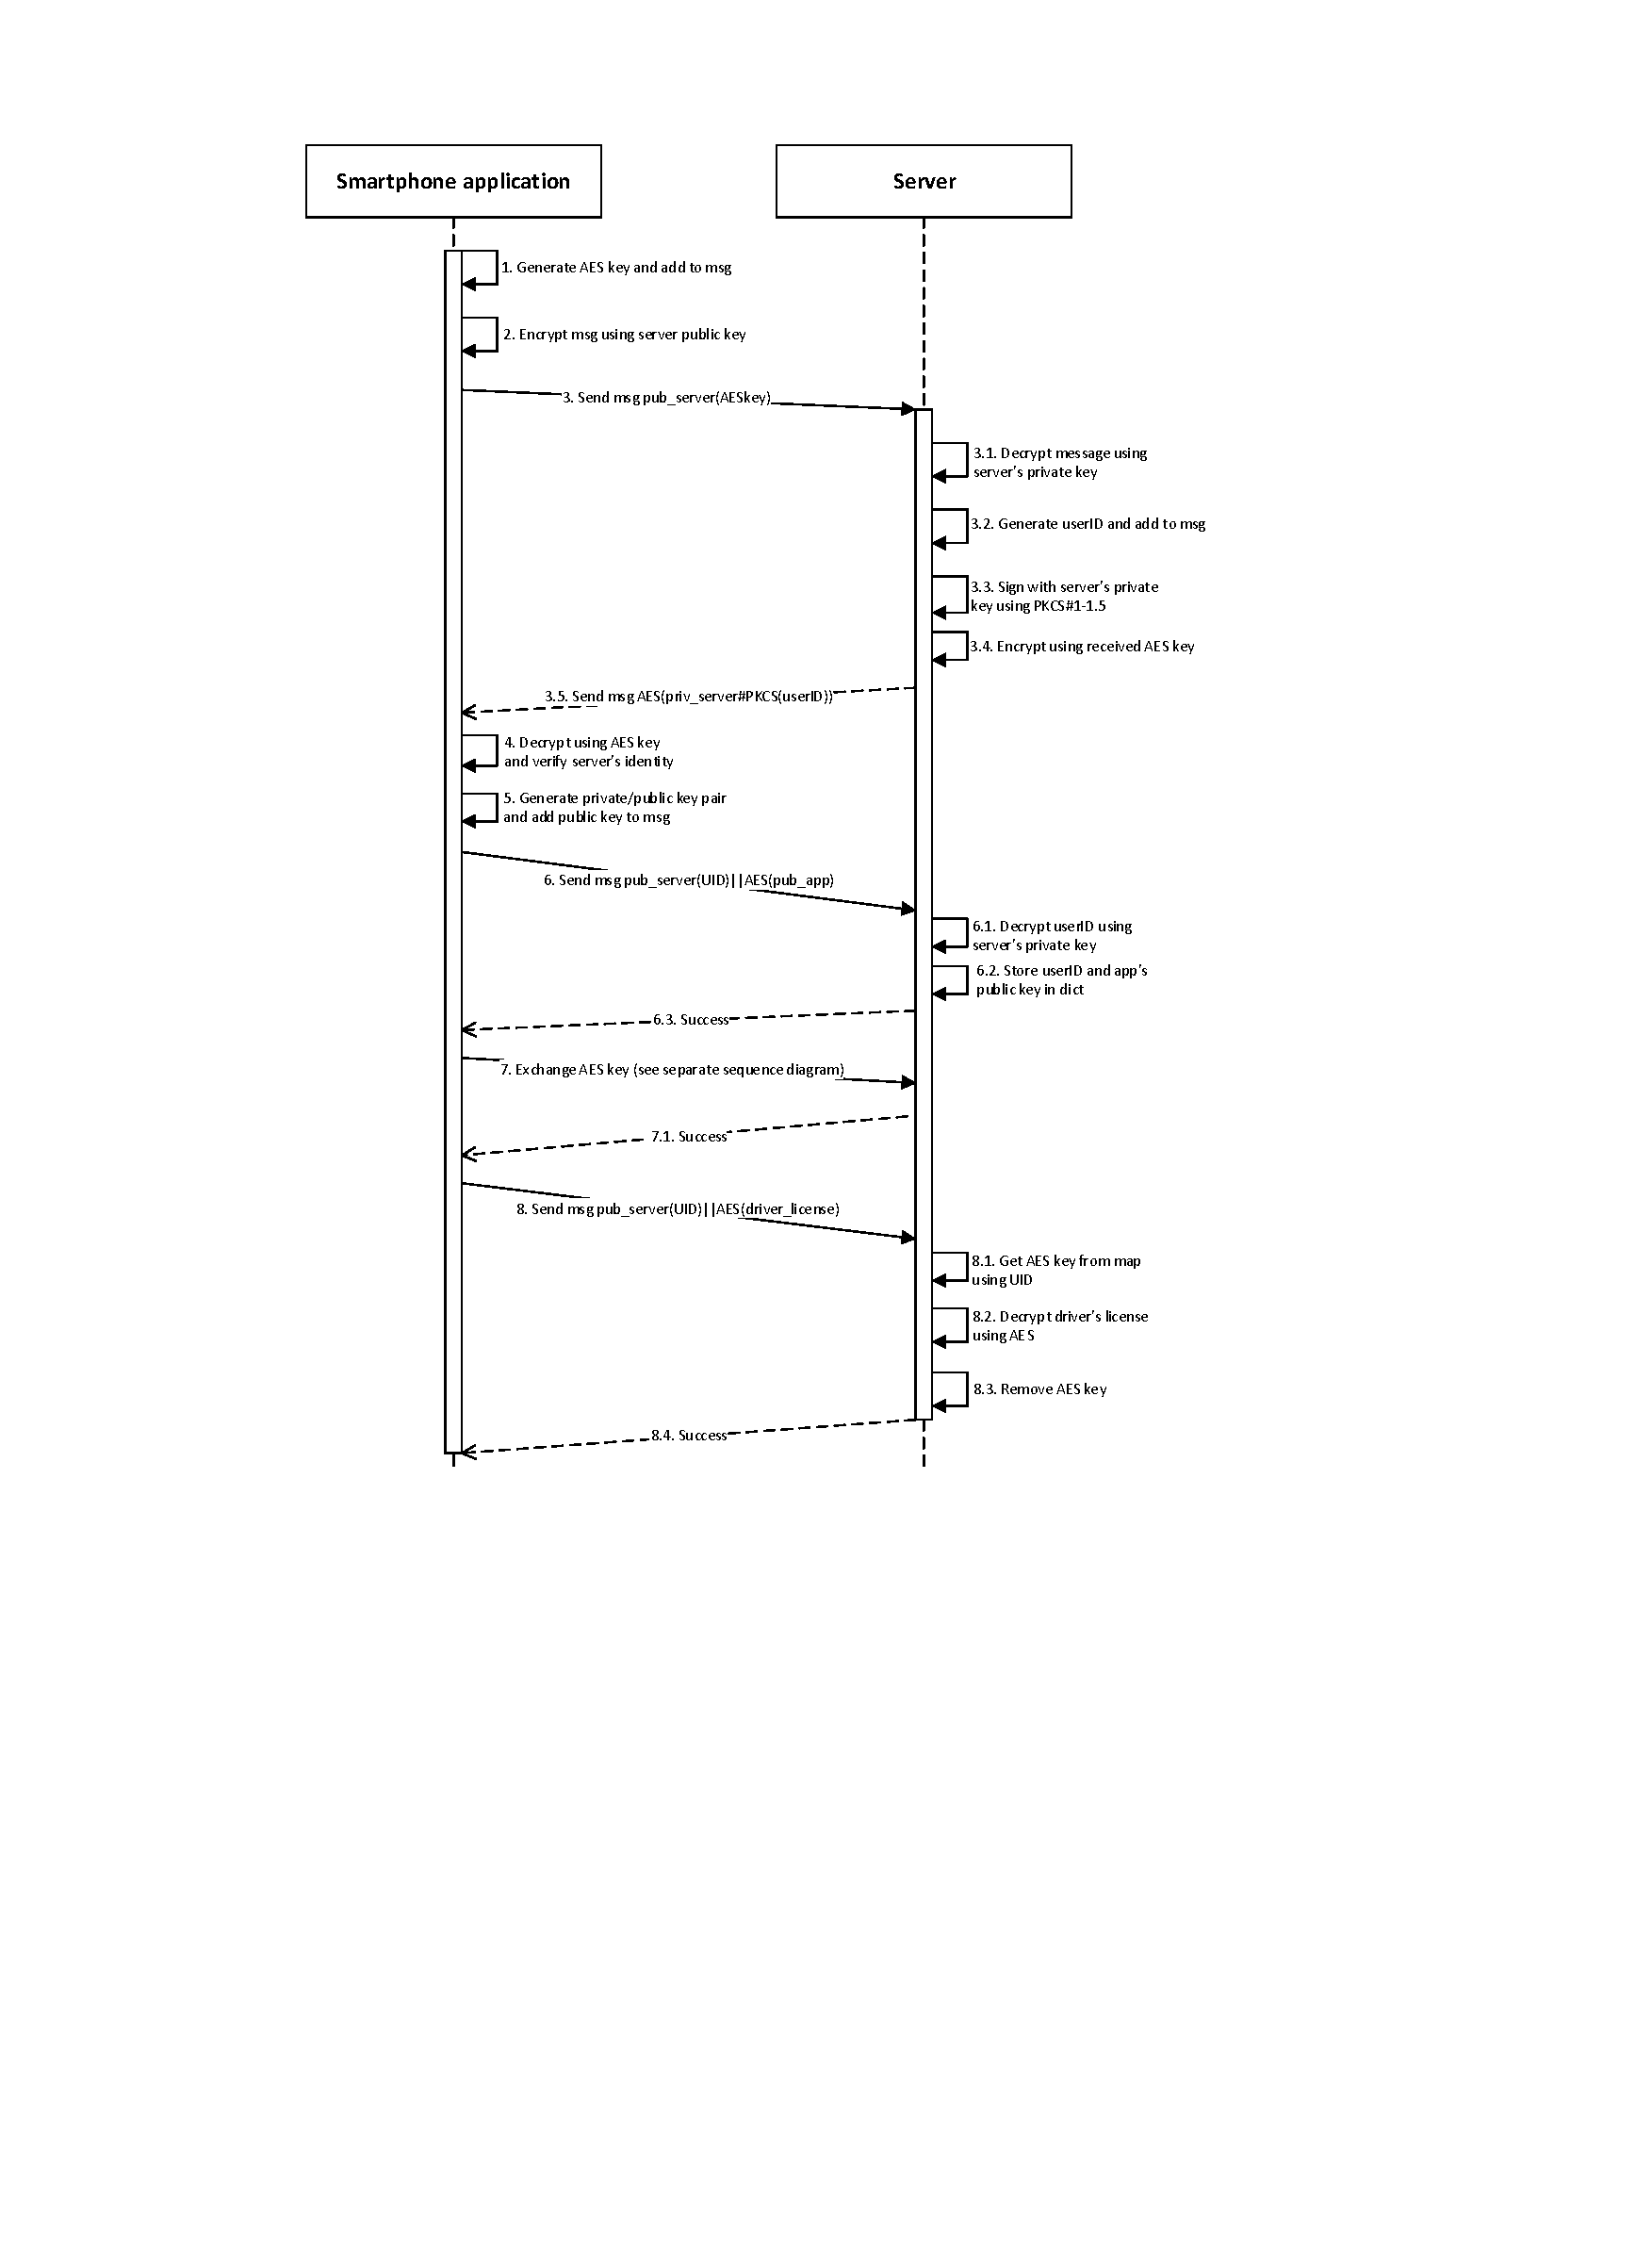
\includegraphics[width=\textwidth, height=.9\textheight,keepaspectratio]{assets/sequencediagram-registration}
\caption{Flow of the registration of a new user, including driver's license check}
\label{fig:sequencediagram-registration}
\end{figure}

\begin{figure}[H]
\centering
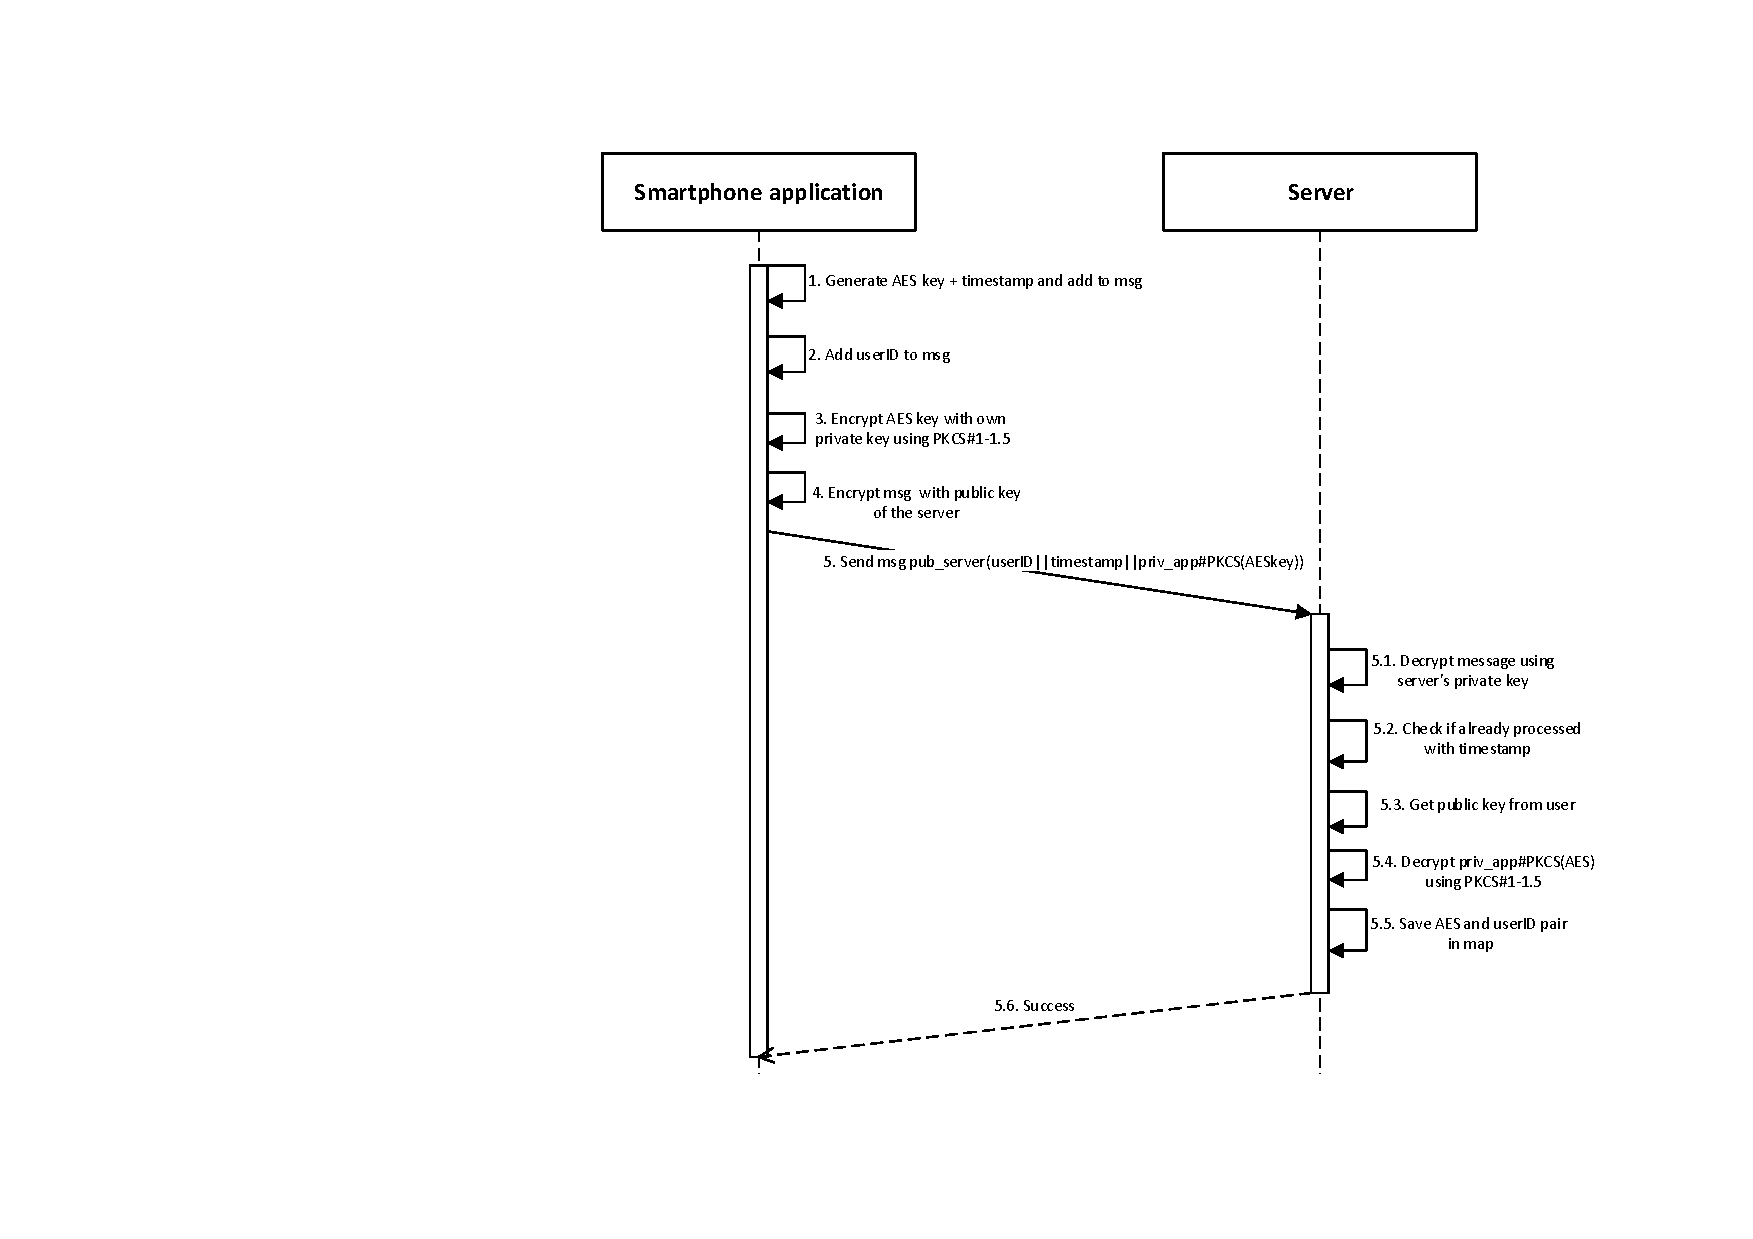
\includegraphics[width=\textwidth]{assets/sequencediagram-keyexchange}
\caption{AES key exchange process between the app and the server}
\label{fig:sequencediagram-keyexchange}
\end{figure}


\begin{figure}[H]
\centering
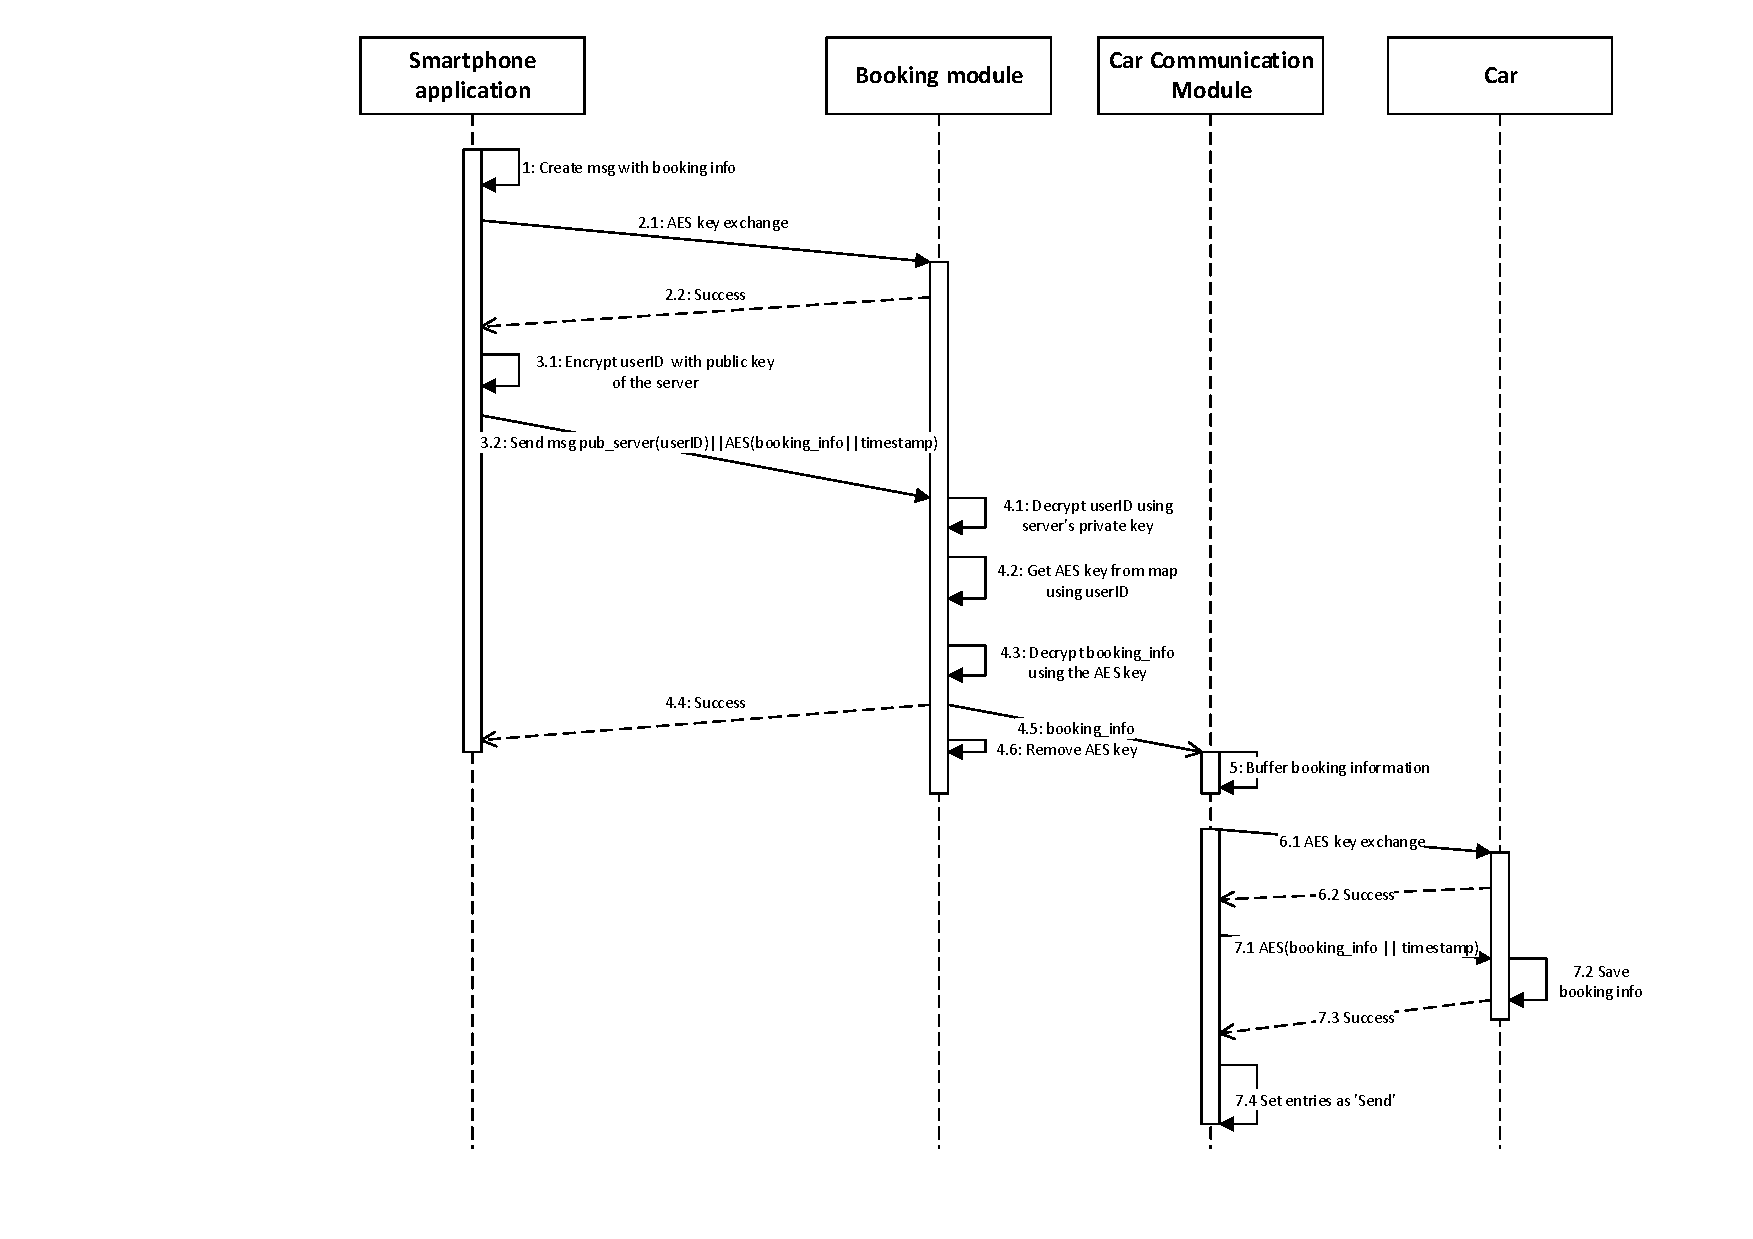
\includegraphics[width=\textwidth]{assets/sequencediagram-booking}
\caption{Flow of the reservation of a car using the smartphone application}
\label{fig:sequencediagram-booking}
\end{figure}


\begin{figure}[H]
\centering
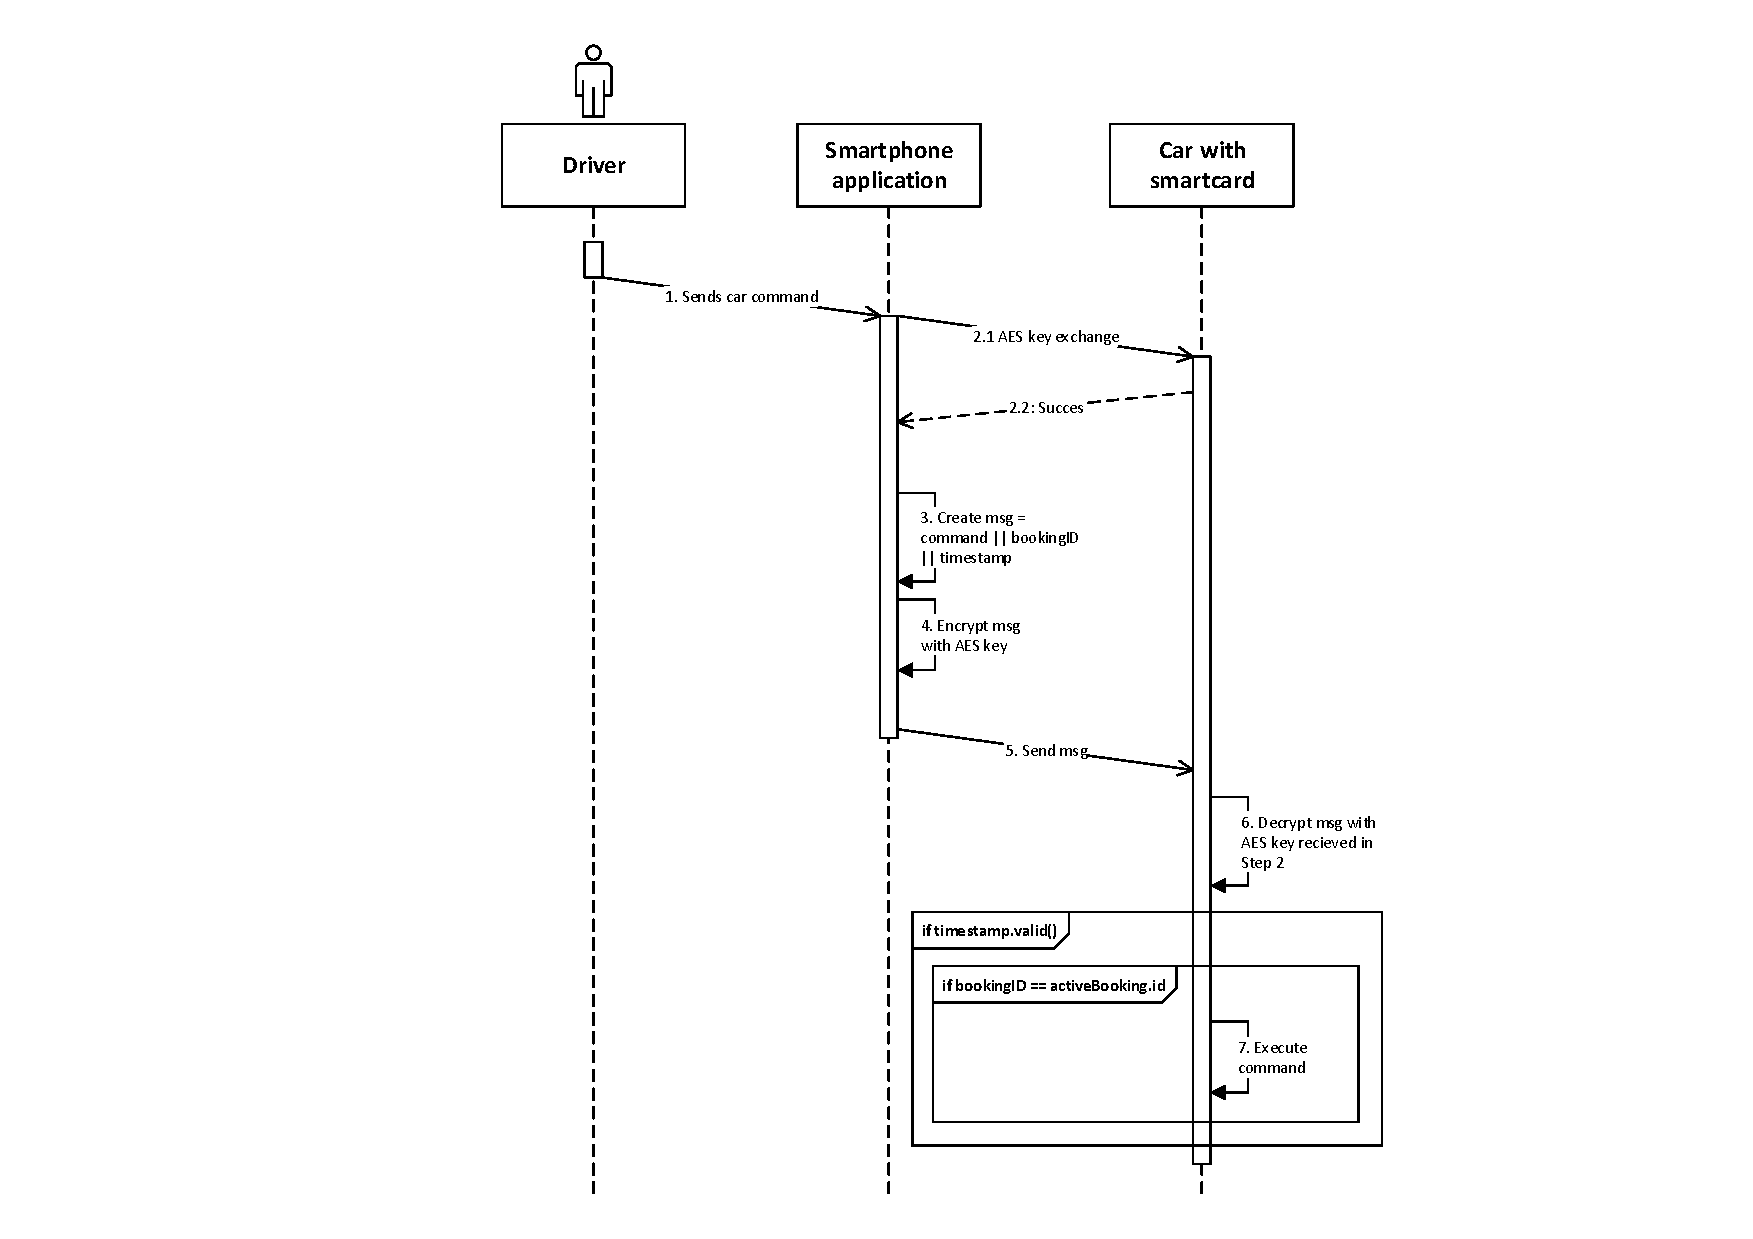
\includegraphics[width=.9\textwidth]{assets/sequencediagram-carcommands}
\caption{Sequence diagram of the car commands use case}
\label{fig:sequencediagram-carcommands}
\end{figure}


\begin{figure}[H]
\centering
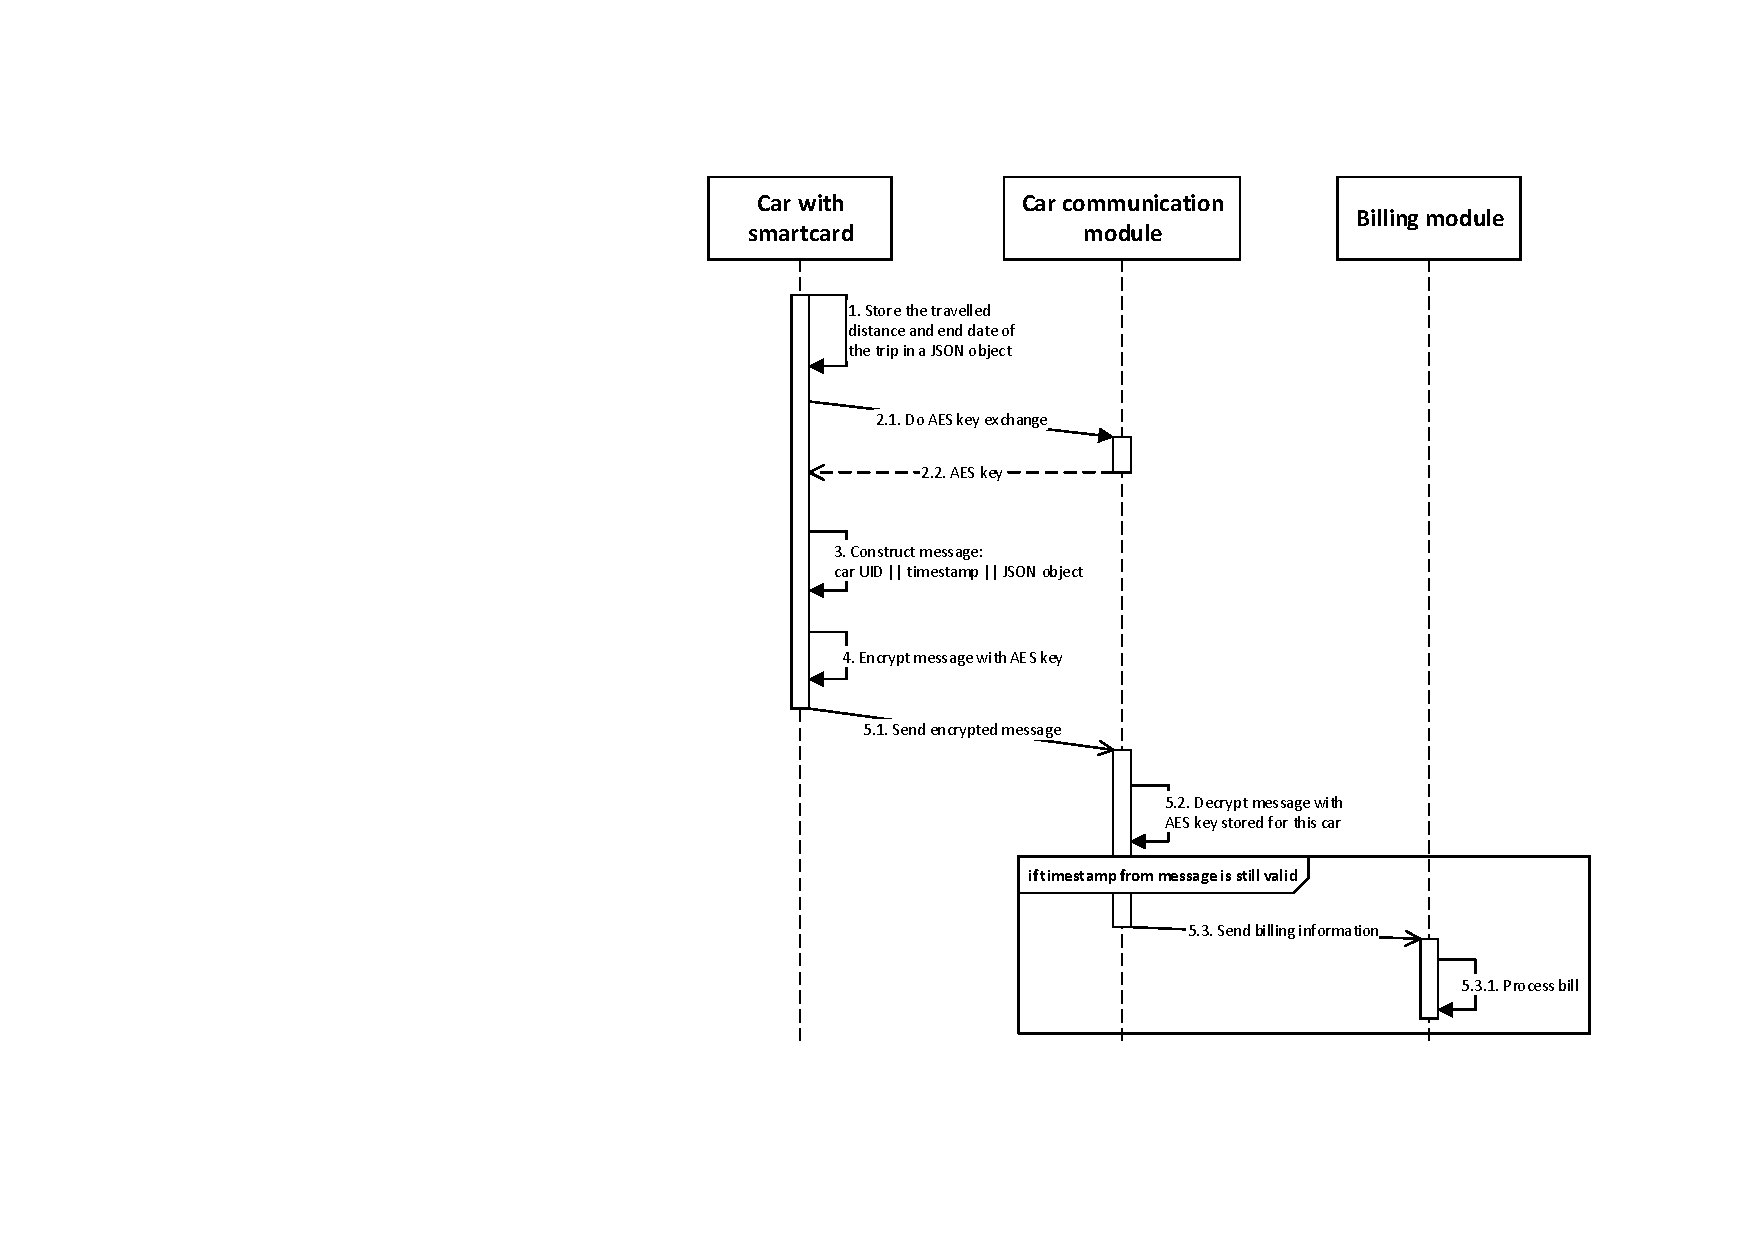
\includegraphics[width=.9\textwidth]{assets/sequencediagram-billing}
\caption{Sequence diagram of the billing use case}
\label{fig:sequencediagram-billing}
\end{figure}

\begin{figure}[p]
  \centering
  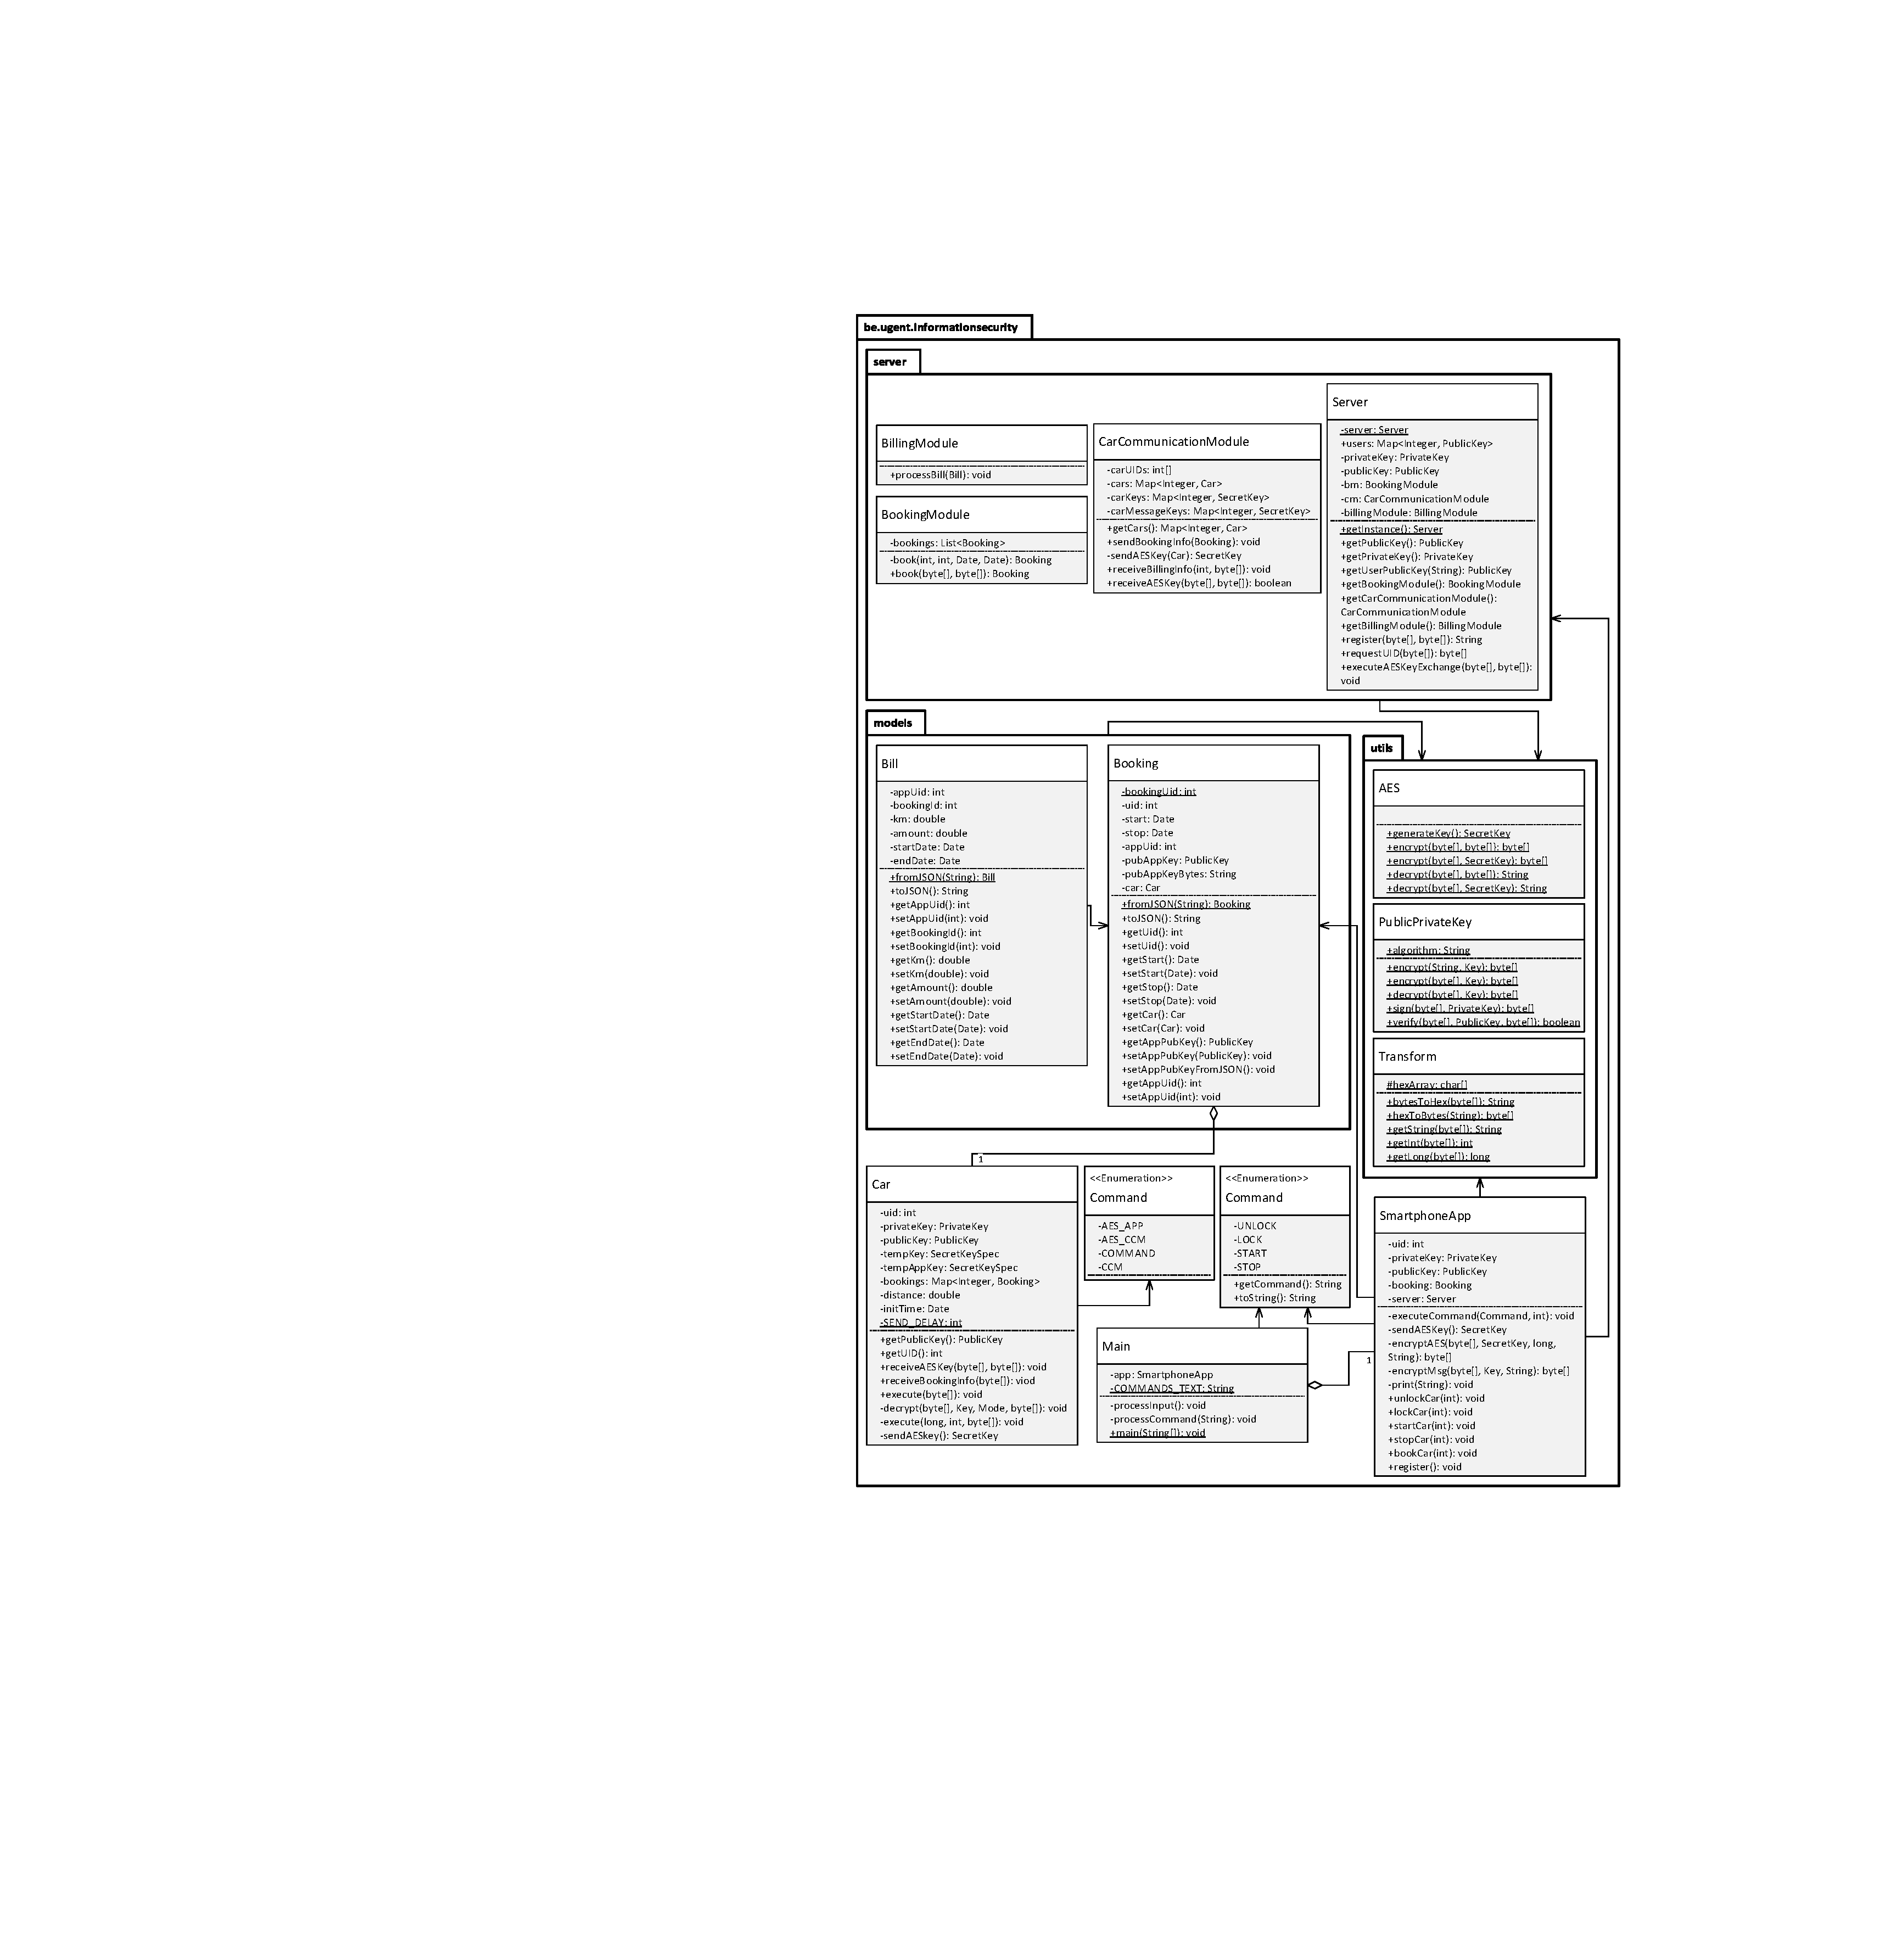
\includegraphics[width=\textwidth, height=.95\textheight, keepaspectratio, origin=c]{assets/architecture-uml}
  \caption{UML class diagram}
  \label{fig:uml-class-diagram}
\end{figure}




%%%%%%%%%%%%%%%%%%%%%%%%%%%%%%%%%%%%%%
\pagebreak
\bibliographystyle{plain} 
\bibliography{references}

\end{document}








